\section{Methodology of DEM Parameter Identification}
\label{sec:methodology}

We now illustrate the methodology used, also shown in Fig.
\ref{fig:19methodology}.
%\begin{figure}[!htb] 
\centering 
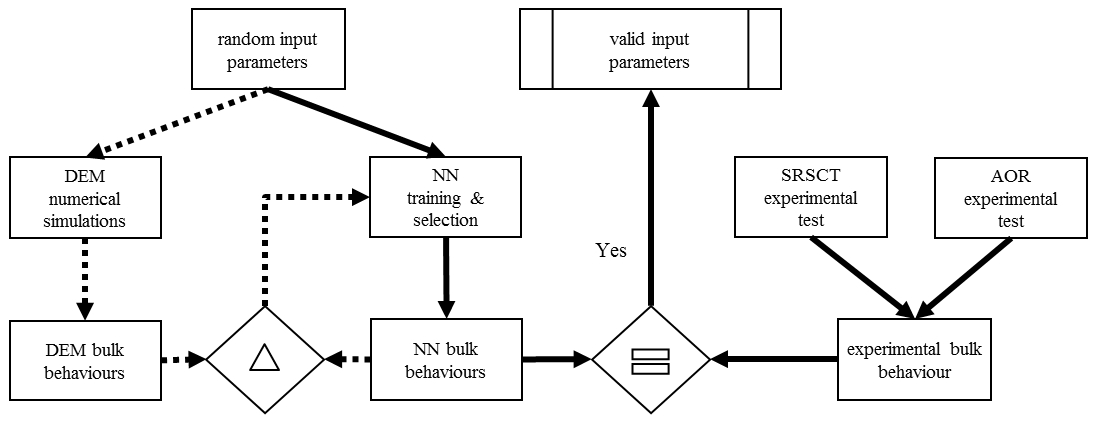
\includegraphics[width=.96\textwidth]{19methodology} 
\caption[Methodology]{Methodology. 
In the training phase (dashed lines) from the initial random input parameters
$DEM$ simulations are performed. The behaviours provided are used to train the
Neural Networks ($NN$), in a loop that continues until the difference is within
the limit ($\Delta$).
Then in the parameters' identification phase (straight
lines) we identify the valid input parameters by comparing (\textbf{=}) $NN$ and
experimental behaviours.
Further explanations in the text.
}
\label{fig:19methodology} 
\end{figure}


% \begin{figure}[htp]
%     \centering
%     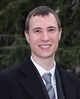
\includegraphics[width=.2\textwidth]{images/vitae/lbenvenuti}
%     \caption{OpenMP, MPI, MPI/OpenMP Hybrid runs of Box in a box testcase on 32
%     cores. The OpenMP-only run suffers from limited memory bandwidth in
%     memory-bound algorithms inside of the Modify section of the code. MPI-only has
%     low averaged runtimes for each section, but a very large Other timing, which
%     hints for a large amount of load-imbalance. Hybrid timings are a bit worse
%     on average, but because of better balancing, processes have lower wait times
%     inside of Other timing.}
% 	\label{fig:boxInBoxComparison}



% After the $DEM$ simulations the Neural
% Network ($NN$) are trained and selected. We then compare experimental and
% numerical results to identify the valid parameters.
The experimental characterization has been performed as described in
\ref{subsec:srsctexperiment} and \ref{subsec:aorexperiment}. We performed
three tests with the $SRSCT$ for the sinter fine bulk, for a total of twelve
load conditions. An example for three of them can be seen in Tab. \ref{tab:05sinterTableExperimental}.
% \begin{table}[h]
\centering
\begin{tabular}{cccccc}
\hline
$\sigma_n$ (Pa) & $\tau$ (Pa) & $\mu_{psh}$ (-) & $\tau_{\%}$ (\%) &
$\mu_{sh}$ (-) & $\rho_b$ (kg/m3) \\
\hline
    1068  & 1059  & 0.9916 & 80 & 1.2333 & 1718 \\
    2069  & 1818  & 0.8787 & 80 & 0.9994 & 1759 \\
    10070 & 8232  & 0.8175 & 80 & 1.1712 & 1802 \\

\hline
\end{tabular}
\caption[Experimental results]{Experimental results. Values for three
load conditions}
\label{tab:05sinterTableExperimental}
\end{table}
The first bulk behaviour representative value ($\rho_b$) is directly provided. 
Concerning the stresses for a sample test, we observed a linear increase in the
coefficient of internal friction, see Fig. \ref{fig:20experimental}.
Later, the first plateau is reached. 
The second bulk behaviour representative value ($\mu_{ie,psh}$) is calculated by averaging the coefficient in this plateau. 
Further, the normal load is modified, and then a second plateau is reached. The third value ($\mu_{ie,sh}$) is 
determined by averaging the coefficient in this plateau. 
Next, we performed two $AOR$ tests. 
Their average provided us the fourth bulk value, allowing us to define the experimental bulk behaviour. 
For simulations purposes, we also sieved the bulk to know the size distribution.
We could then focus on the numerical section of the characterization. 
As stated in the modelling section of this paper, we decided to fix one univocal contact law for all the simulations performed. 
Furthermore, we locked the size distribution, as provided by the sieving, the
elastic coefficients and the time step, see Tab.
\ref{tab:09DEMFixedinputvalues}.
% \begin{table}[h]
\centering
\begin{tabular}{ccc}
\hline
    Young's & Poisson's & \acs{deltat}\\
   modulus & ratio & \\
    $[MPa]$ & $[-]$ & [s]\\
    \hline
    $10$    & $0.40$ & $10^{-6}$\\


\hline
\end{tabular}
\caption{DEM fixed input values}
\label{tab:09DEMFixedinputvalues}
\end{table}
% \begin{table}[h]
\centering
\begin{tabular}{ccccc}
\hline
    \acs{mus} & \acs{mur} & \acs{CoR} & \acs{rhop} & \acs{dCylDp} \\
    	$[-]$  & $[-]$   & $[-]$   & $[kg/m3]$ & $[-]$ \\
    \hline
    0.4 / 0.6 / 0.8 & 0.4 / 0.6 / 0.8 & 0.5 / 0.7 / 0.9 & 2500 / 3000 / 3500 & 20 / 36 / 38 / 40 \\

\hline
\end{tabular}
\caption[DEM variable input values]{DEM variable input values for training the
Neural Networks}
\label{tab:10DEMVariableinputvalues}
\end{table}
The latter was smaller than the Rayleigh time. Instead, $COR$, $\mu_s$, $\mu_r$,
$\rho_p$ and $dCylDp$, as indicated in Tab. \ref{tab:10DEMVariableinputvalues},
were constant in each simulation, but their combination differed between
simulations, see e.g. Tab. \ref{tab:11DEMSimExampleinputvalues}.
% \begin{table}[h]
\centering
\begin{tabular}{lccccc}
\hline
 sim &  $\mu_s$ & $\mu_r$ & $COR$ & $\rho_p$ & $dCylDp$ \\
  \#  &	$[-]$  & $[-]$   & $[-]$   & $[kg/m3]$ & $[-]$ \\
          \hline
    1st & 0.40  & 0.40  & 0.50  & 2500  & 20 \\
    2nd & 0.60  & 0.40  & 0.50  & 2500  & 20 \\


\hline
\end{tabular}
\caption{DEM simulation examples input values}
\label{tab:11DEMSimExampleinputvalues}
\end{table}
Further, $dCylDp$ was used to evaluate the wall effect, but only $~10\%$ of the
all simulations had $dCylDp$ larger than $20$. The normal stress $\sigma_n$ and its
percentage during the incipient flow condition $\tau_{\%}$
varied to replicate the twelve shear cell load conditions. 
In total, we realized $546$ shear cell and $81$ angle of repose simulations.
A Matlab script allowed us to extract from the simulations output the numerical
bulk representative values ($\mu_{ie-ps}$, $\mu_{ie-s}$, $\rho_b$ and $AOR$) for each $simulation-DEM$ parameter combination. 
So, we could use the $DEM$ parameter combinations and their corresponding bulk values to train the $NN$. 
Notably, we excluded 15\% of the simulations ($test ~ simulations$), casually
picked, from the training processes.
First, we started with all the $DEM$ parameter combinations and their corresponding numerical $\mu_{ie-ps}$ to create 36 $NN$. 
They differed because they have from five to forty neurons in the hidden layer. 
Later, we controlled the square regression error between the $bulk-macro$ behaviours in the output of 
the $NN$ and the 15\% $test ~ simulations$, granted uncorrelated. 
So, we could select for $\mu_{ie-ps}$ the $NN$ with the maximum $R^2$, and we noted its number of neurons. 
We repeated the same steps from the $NN$ creations for $\mu_{ie-s}$, $\rho_b$ and $AOR$, 
obtaining one trained $NN$ for each bulk representative value. \\
% \begin{table}[h]
\centering
\begin{tabular}{lcccc}
\hline
 &  \ac{mus} & \ac{mur} & \ac{CoR} & \ac{rhop}  \\
  &	$[-]$  & $[-]$   & $[-]$   & $[kg/m3]$ \\
          \hline
    range & $[0.1 \ldots 1.0]$ & $[0.1 \ldots 1.0]$ & $[0.5 \ldots 0.9]$ &
    $[2000 \ldots 3500]$     \\
    \# rnd & 100   & 100   & 25    & 25    \\

\hline
\end{tabular}
\caption[DEM random input values]{DEM random input values. Within each range \#
random values are chosen.}
\label{tab:12DEMRandominputvalues}
\end{table}
Since $\mu_{ie-ps}$, $\mu_{ie-s}$ and $\rho_b$ belonged to the shear cell
simulations their $NN$ were handled together. We then created random values in the range
and number defined in Tab. \ref{tab:12DEMRandominputvalues}.
The total number of combinations of these random values was $6250000$. These
combinations were then processed by the selected $NN$, granting for each three bulk representative parameters for the shear cell and one for the $AOR$. Later, we confronted the $NN$ and experimental bulk behaviours for the twelve shear cell load conditions. 
If in a $DEM-parameter$ combination all the three bulk representative parameters differed less 
than 5\% from the corresponding experiments, see Eq. \ref{eq:check2}:
\begin{equation}
 \begin{cases}
\text{if } & \lvert{1-\frac{\mu_{psh,num}}{\mu_{psh,exp}}}\rvert < 5\%  ,\\
\text{and if } & \lvert{1-\frac{\mu_{sh,num}}{\mu_{sh,exp}}}\rvert < 5\% , \\ 
\text{and if } & \lvert{1-\frac{\rho_{p,num}}{\rho_{p,exp}}}\rvert < 5\% ,\\ 
\end{cases}
 \label{eq:check2}
\end{equation}
then the combination was tabbed. The latter combinations were handled by the $AOR$ $NN$, and then confronted with the experiment. 
Only those that differed less than $5\%$ also in this comparison (Eq.
\ref{eq:checkaor}) were branded as valid:
\begin{equation}
\text{if} ~~~~~~ \lvert{1-\frac{AoR_{num}}{AoR_{exp}}}\rvert < 5\% .
\label{eq:checkaor}
\end{equation}
%************************************************
Further, to prove the system validity, we tested the tabbed combinations by modifying the experimental bulk
behaviour representative values of the shear cell. 
We artificially decreased or increased all of them by a product coefficient ($P$).
\begin{figure}[!htb] 
\centering 
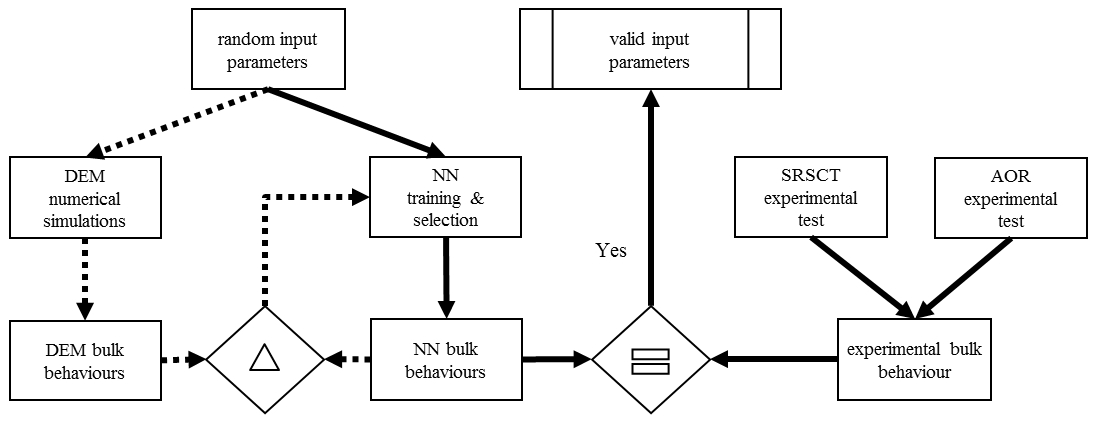
\includegraphics[width=.96\textwidth]{19methodology} 
\caption[Methodology]{Methodology. 
In the training phase (dashed lines) from the initial random input parameters
$DEM$ simulations are performed. The behaviours provided are used to train the
Neural Networks ($NN$), in a loop that continues until the difference is within
the limit ($\Delta$).
Then in the parameters' identification phase (straight
lines) we identify the valid input parameters by comparing (\textbf{=}) $NN$ and
experimental behaviours.
Further explanations in the text.
}
\label{fig:19methodology} 
\end{figure}


% \begin{figure}[htp]
%     \centering
%     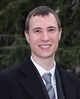
\includegraphics[width=.2\textwidth]{images/vitae/lbenvenuti}
%     \caption{OpenMP, MPI, MPI/OpenMP Hybrid runs of Box in a box testcase on 32
%     cores. The OpenMP-only run suffers from limited memory bandwidth in
%     memory-bound algorithms inside of the Modify section of the code. MPI-only has
%     low averaged runtimes for each section, but a very large Other timing, which
%     hints for a large amount of load-imbalance. Hybrid timings are a bit worse
%     on average, but because of better balancing, processes have lower wait times
%     inside of Other timing.}
% 	\label{fig:boxInBoxComparison}



% After the $DEM$ simulations the Neural
% Network ($NN$) are trained and selected. We then compare experimental and
% numerical results to identify the valid parameters.
\begin{table}[h]
\centering
\begin{tabular}{cccccc}
\hline
$\sigma_n$ (Pa) & $\tau$ (Pa) & $\mu_{psh}$ (-) & $\tau_{\%}$ (\%) &
$\mu_{sh}$ (-) & $\rho_b$ (kg/m3) \\
\hline
    1068  & 1059  & 0.9916 & 80 & 1.2333 & 1718 \\
    2069  & 1818  & 0.8787 & 80 & 0.9994 & 1759 \\
    10070 & 8232  & 0.8175 & 80 & 1.1712 & 1802 \\

\hline
\end{tabular}
\caption[Experimental results]{Experimental results. Values for three
load conditions}
\label{tab:05sinterTableExperimental}
\end{table}
\begin{table}[h]
\centering
\begin{tabular}{ccc}
\hline
    Young's & Poisson's & \acs{deltat}\\
   modulus & ratio & \\
    $[MPa]$ & $[-]$ & [s]\\
    \hline
    $10$    & $0.40$ & $10^{-6}$\\


\hline
\end{tabular}
\caption{DEM fixed input values}
\label{tab:09DEMFixedinputvalues}
\end{table}
\begin{table}[h]
\centering
\begin{tabular}{ccccc}
\hline
    \acs{mus} & \acs{mur} & \acs{CoR} & \acs{rhop} & \acs{dCylDp} \\
    	$[-]$  & $[-]$   & $[-]$   & $[kg/m3]$ & $[-]$ \\
    \hline
    0.4 / 0.6 / 0.8 & 0.4 / 0.6 / 0.8 & 0.5 / 0.7 / 0.9 & 2500 / 3000 / 3500 & 20 / 36 / 38 / 40 \\

\hline
\end{tabular}
\caption[DEM variable input values]{DEM variable input values for training the
Neural Networks}
\label{tab:10DEMVariableinputvalues}
\end{table}
\begin{table}[h]
\centering
\begin{tabular}{lccccc}
\hline
 sim &  $\mu_s$ & $\mu_r$ & $COR$ & $\rho_p$ & $dCylDp$ \\
  \#  &	$[-]$  & $[-]$   & $[-]$   & $[kg/m3]$ & $[-]$ \\
          \hline
    1st & 0.40  & 0.40  & 0.50  & 2500  & 20 \\
    2nd & 0.60  & 0.40  & 0.50  & 2500  & 20 \\


\hline
\end{tabular}
\caption{DEM simulation examples input values}
\label{tab:11DEMSimExampleinputvalues}
\end{table}
\begin{table}[h]
\centering
\begin{tabular}{lcccc}
\hline
 &  \ac{mus} & \ac{mur} & \ac{CoR} & \ac{rhop}  \\
  &	$[-]$  & $[-]$   & $[-]$   & $[kg/m3]$ \\
          \hline
    range & $[0.1 \ldots 1.0]$ & $[0.1 \ldots 1.0]$ & $[0.5 \ldots 0.9]$ &
    $[2000 \ldots 3500]$     \\
    \# rnd & 100   & 100   & 25    & 25    \\

\hline
\end{tabular}
\caption[DEM random input values]{DEM random input values. Within each range \#
random values are chosen.}
\label{tab:12DEMRandominputvalues}
\end{table}